\documentclass{article}
\usepackage[utf8]{inputenc}
\usepackage[english]{babel}
\usepackage{amsmath}
\usepackage{amssymb}
\usepackage{physics}
\usepackage{nicefrac}
\usepackage{graphics}
\usepackage{graphicx}
\usepackage{subfig}
\usepackage{svg}
\usepackage{pdfpages}
\usepackage{placeins}
\usepackage[a4paper, top=2cm, bottom=2.5cm, left=3cm, right=3cm]{geometry}
\usepackage[colorlinks=true, urlcolor=blue, linkcolor=blue]{hyperref}
\usepackage{siunitx}
\sisetup{
	locale = UK,
	per-mode = fraction,    
	separate-uncertainty
}
\usepackage{comment}
\usepackage{float}
\usepackage{dsfont}

\newcommand{\namen}{Fabian Ganzer}
\newcommand{\headline}{IST research project: \\Rejection of matrix elements in the coupling matrix of an Ising model for active user detection}

\hypersetup{pdfauthor=\namen, pdftitle=\headline}

\title{\headline}
\author{\namen }

\date{\begin{tabular}{ll}
		Time period:  & winter semester 2024/2025         \\
		Institution:      & INSA Lyon, CITI laboratory          \\
		Supervisors: &  Prof.~Claire Goursaud, Romain Piron	          \\
\end{tabular}}



\begin{document}
	\maketitle 
	\begin{abstract}
		To solve the active user detection problem, a quantum annealer can be used. To mitigate the effect of noise leading to a degraded accuracy, the original problem can be simplified by rejecting couplings in the coupling matrix of the Ising model. In this project, three methods for the rejection of those matrix elements are studied.
	\end{abstract}
	\tableofcontents
	\newpage
	
	\section{Introduction}
	In 6G wireless networks, resources like frequency or time slots are only allocated to active devices. Consequently, it is necessary to identify which devices are active. This task is known as active user detection (AUD). If a non-orthogonal medium access technique is employed to identify users, interference between the identification sequences, the so-called pilot sequences, is introduced. To detect the active users in this case, a maximum likelihood estimator can be used, which however needs an exponentially increasing time with a growing number of users. \cite{PirGou1}
	
	Luckily, the mathematical formulation thereof can be mapped to an Ising Hamiltonian which allows to solve the active user detection problem using a quantum annealer promising a significant speedup. This however raises practical problems of accuracy. The larger the problem gets one is trying to solve, the more qubits are necessary, the more problematic the noise gets and therefore the more the accuracy decreases. 
	
	Our approach to mitigate these effects is to modify the problem in advance in order to reduce the number of necessary qubits. This modification is expected to reduce the influence of noise during the annealing process, however it introduces new errors because the problem itself is simplified and therefore it is not anymore equivalent to the problem one is actually trying to solve. If however the modifications are small, the results obtained by solving the simplified version of the problem might still be useful for the original, non-simplified version of the problem. The overarching goal would thus be to answer the following question: Does one reach a higher rate of correct active user detections by simplifying the problem, thus having less noise but thereby introducing errors in the problem itself or is it more favorable to stick to the original, more complex problem without any errors however having to accept more noise during the annealing process?
	
	This work aims to progress on one part of this overarching question. It focuses only on the errors that are introduced by the modification of the problem. This means, an ideal annealing process without any noise is considered.  
	
	This work begins by a presentation of the used system model in Sec.~\ref{sec:system model} followed by an introduction of the methods used for simplifying the problem in Sec.~\ref{sec:methods for rejection of couplings}. Sec.~\ref{sec:hamming distance} to Sec.~\ref{sec:dependence on the connectedness of the graph} focus on the examination of certain relationships between the parameters describing the amount of problem modification and figures of merit like the ratio of correct detections, followed by a comparison of all three modification methods in Sec.~\ref{sec:comparison of rejection methods}.
	
	\section{System model}\label{sec:system model}
	The system model used for this work is the same as the one presented in Ref.~\cite{PirGou1}.
	
	$N$ users are part of a network, each being assigned a pilot sequence $\vec p_n\in\mathbb{C}^M$, normalized such that $||\vec p_n||=1$. The activity pattern $\alpha^{(0)}$ represents which user is active and which one is inactive and is defined as 
	\begin{equation}
		\alpha_n^{(0)} =\begin{cases}
			1 \quad\text{if $n$-th user is active} \\ 0\quad\text{otherwise}
		\end{cases}, \quad n=1,...,N.
	\end{equation}
	The goal is to recover this activity pattern from a received signal. The signal is received at $K$ antennas and the channel between user $n$ and all $K$ antennas is modeled by Rayleigh fading such that $\vec h_n \sim \mathcal{N}(0,\mathds{1}_K)$, where $\mathds{1}_K$ designates the $K\times K$ unit matrix. Each antenna is impacted by additive white gaussian noise (AWGN) $\vec w_k\sim\mathcal{N}(0, \xi^2\mathds{1}_M)$ where $\xi$ is a parameter controlling the strength of the noise. The signal received at antenna $k$ thus reads
	\begin{equation}
		\vec y_k = \sum\limits_{n=1}^N \alpha_n^{(0)} \vec p_n (\vec h_n)_k + \vec{w}_k.
	\end{equation}
	To consider all antennas together, one introduces the following matrix notation:
	\begin{align}
		P &= \bigl(\vec p_1...\vec p_N\bigr)\in\mathbb{C}^{M\times N} &\text{ (Pilot matrix)}\\
		H &= \bigl(\vec h_1...\vec h_N\bigr)\in\mathbb{C}^{K\times N} &\text{ (Channel matrix)}\\
		W &= \bigl(\vec w_1...\vec w_N\bigr)\in\mathbb{C}^{M\times K} &\text{ (AWGN)}
	\end{align}
	to write the matrix $Y\in\mathbb{C}^{M\times K}$ as
	\begin{equation}
		Y = \sum\limits_{n=1}^N\alpha_n^{(0)}\vec p_n\vec h_n^T + W = P\cdot \mathrm{Diag}(\alpha^{(0)})\cdot H + W
	\end{equation}
	In this project, only the scenario without AWGN noise, i.e. $\xi=0$ is considered. 
	
	To find the activity pattern, we introduce the covariance matrix
	\begin{equation}
		\hat{\Sigma}_Y = \frac{1}{K}\sum\limits_{k=1}^K\vec y_k \vec y_k^\dagger = \frac{1}{K}YY^\dagger
	\end{equation}
	from which we can determine the estimator $\alpha$ of the activity pattern $\alpha^{(0)}$ using a least squares approach:
	\begin{equation}
		\alpha = \underset{\tilde{\alpha}\in\{0,1\}^N}{\arg\min}||P\cdot\mathrm{Diag}(\tilde{\alpha})\cdot P - \hat{\Sigma}_Y||_F^2.
	\end{equation}
	Using the spin configuration $\vec\sigma = 1-2\vec\alpha$, this expression can be mapped to to the Ising model
	\begin{equation}
		H_P = -\sum\limits_{i<j}J_{ij}\sigma_i\sigma_j - \sum_i b_i\sigma_i,
	\end{equation}
	where the couplings $J_{ij}$ and the local fields are given by
	\begin{align}
		J_{ij} &= -\frac{1}{2}|\vec p_i^\dagger \vec p_j|^2 \\
		b_i &= -\Tr(\vec p_i\vec p_i^\dagger\hat{\Sigma}_Y)+\frac{1}{2}\sum\limits_{j=1}^N|\vec p_i^\dagger \vec p_j|^2.
	\end{align}
	The solution $\alpha$ can be obtained by measuring the ground state of the Ising Hamiltonian, called problem Hamiltonian, and converting the spin variables using $\vec \alpha = \frac{1+\vec\sigma}{2}$. The system can be caused to adopt the ground state of the Ising Hamiltonian by the use of quantum annealing. This means, that the system is prepared in the ground state of a Hamiltonian whose ground state is known, typically called the control Hamiltonian, and then adiabatically evolved towards the system described by the problem Hamiltonian. In this project however, we consider an ideal annealing process, meaning that it is not necessary to simulate the whole annealing process. Instead, it is faster to obtain the solution by an exhaustive search among all possible basis states. This means that the energy given by the problem Hamiltonian is evaluated for all possible basis states and the basis state with the lowest energy represents the solution. 
	
	The parameters used for this project are always $N=5, M=4, K=100, \xi=0$.
	
	\section{Methods for rejection of couplings}\label{sec:methods for rejection of couplings}
	The goal of this project is to examine the rejection of couplings in the Ising model for active user detection. This raises the question how to neglect the couplings. In this project, three different methods are considered. 
	\paragraph{Threshold method.} Small couplings are expected to only contribute little to the overall outcome of the annealing process. Thus, it is reasonable to neglect those. In order to do so, a threshold $\eta$ is introduced and a coupling $J_{ij}$ is rejected, if its absolute value is smaller than the threshold $\eta$, or mathematically speaking, the modified coupling matrix $\tilde{J}$ is obtained from the coupling matrix $J$ by:
	\begin{equation}
		\tilde{J}_{ij} = \begin{cases}
			0 \quad\text{if}\quad |J_{ij}|<\eta \\ J_{ij} \quad\text{otherwise} 
		\end{cases}.
	\end{equation}
	
	\paragraph{Number method.} The second method fixes a total number allowed for the couplings. Starting from the smallest coupling, couplings are rejected in rising order as long as the total number of couplings is larger than a maximally allowed number $N_c^\text{max}$. Mathematically, we get
	\begin{equation}
		\tilde{J}_{ij}^{(l+1)} = \begin{cases}
			0 \quad\text{if}\quad |\{\tilde{J}_{ij}^{(l)}|\tilde{J}_{ij}^{(l)}\neq0\}|>N_c^\text{max} \\ J_{ij} \quad\text{otherwise} 
		\end{cases},
	\end{equation}
	where the upper index indicates the number of iterations such that $l=0$ indicates the iteration with the matrix element of smallest magnitude.

	\paragraph{Degree method.}In a real quantum annealer, for instance the ones by D-Wave, the criterion for implementation of a certain Ising model, is the physical implementation that is already given by the company. This means, each qubit only has a certain number of couplings that are maximally allowed. This motivates the introduction of the degree method. For this method, the goal is to reject couplings such that the modified problem only involves qubits whose number of couplings does not exceed a certain maximum number, i.e. the corresponding graph has only nodes whose degree is equal or less to a certain maximum degree. The implementation used here is as follows: One iterates over all couplings starting with the smallest non-zero coupling in the matrix $J$. This coupling connects two qubits. If either one of them has a degree that exceeds a certain maximum degree $\delta$, the respective coupling is rejected. As an equation, this means
	\begin{equation}
		\tilde{J}_{ij}^{(l+1)} = \begin{cases} 0 \quad\text{if}\quad \mathrm{deg}(i^{(l)})>\delta \quad \text{and}\quad \mathrm{deg}(j^{(l)})>\delta \\
			J_{ij} \quad\text{otherwise}
		\end{cases}.
	\end{equation}
	
	
	\section{Hamming distance}\label{sec:hamming distance}
	The goal of the annealing process is to recover the activity pattern. Due to the modification of the coupling matrix, one changes the problem that is going to be solved leading to bit errors in the activity pattern. How strong the deviation of the determined activity pattern from the actual activity pattern is, can be quantified using the hamming distance $d_\text{H}$.
	To investigate, how strong this effect is, many problem instances are generated, matrix elements rejected according to the threshold method and the ground state is determined. This is repeated for different rejection thresholds.
	 
	\begin{figure}[h]
		\begin{minipage}{0.49\textwidth}
			\centering
			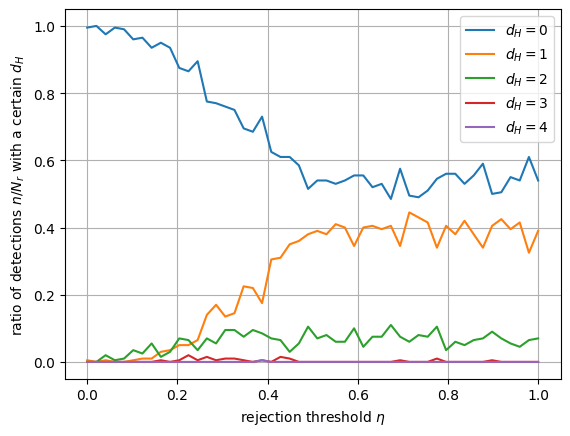
\includegraphics[width=\textwidth]{img/hamming_rule_1.png}
			\caption{average number of neglected couplings}
			\label{fig:hamming rule 1}
		\end{minipage}
		\begin{minipage}{0.49\textwidth}
			\centering
			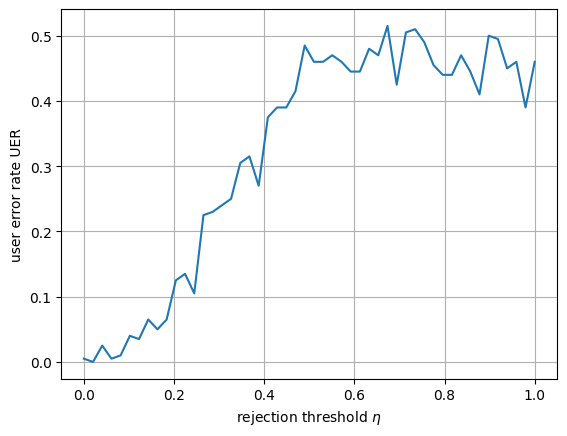
\includegraphics[width=\textwidth]{img/uer_rule_1.png}
			\caption{average number of connected graphs}
			\label{fig:uer rule 1}
		\end{minipage}	
	\end{figure}
	The results are shown in Fig.~\ref{fig:hamming rule 1}. A hamming distance of $d_\text{H}=0$ means that the initial activity pattern is recovered without any bit errors. As expected, this curve starts close to 1 for $\eta=0$ because in that case, the problem isn't modified. With increasing rejection threshold, the percentage of correct detections drops. Until $\eta=0.2$, the steepness seems to increase, followed by a linear descent. After $\eta=0.5$, the ratio rests on a plateau around 0.5. This means that in 50\,\% of the cases, the initial activity pattern is recovered correctly. The curves for the other hamming distances, start at 0 and increase to a plateau starting at around $\eta=0.5$. The higher the hamming distance, the fewer occurrences there are, which is valuable information because this means, that bit errors where many bits are flipped, are relatively unlikely. In fact, in the regime of the plateau, where around 50\,\% of the problems are solved correctly, 40\,\% of the cases yield just a single bit error. This on the other hand means, that in 90\,\% of the cases, there is {\it at most} one bit error. 
	
	Another typical way of presenting the accuracy of such detection processes, is the user error rate (UER). It is defined as 
	\begin{equation}
		UER = \frac{|\{\text{wrong bits in $\alpha$}\}|}{N}
	\end{equation}
	and presented in Fig.~\ref{fig:uer rule 1}. As it is the sum of the occurrences of all hamming distances greater than 0, it shows a similar behavior as the graphs in Fig.~\ref{fig:hamming rule 1}. 
	
	
	\begin{figure}[h]
		\begin{minipage}{0.49\textwidth}
			\centering
			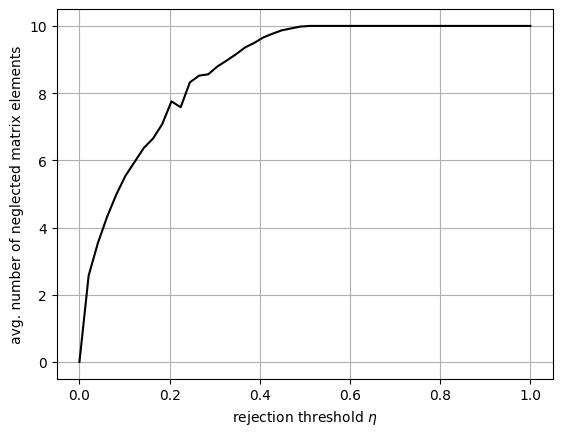
\includegraphics[width=\textwidth]{img/N_neglected_rule_1.png}
			\caption{average number of neglected couplings}
			\label{fig:N neglected rule 1}
		\end{minipage}
		\begin{minipage}{0.49\textwidth}
			\centering
			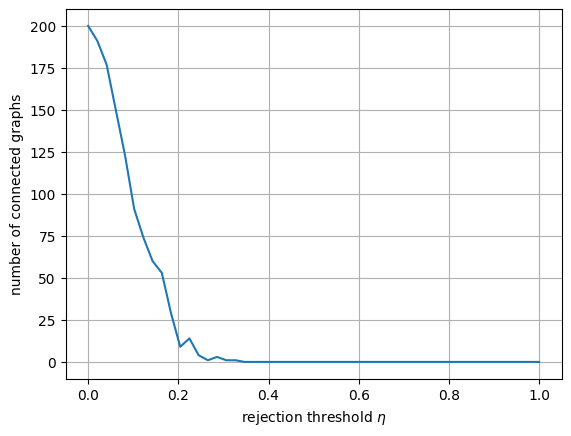
\includegraphics[width=\textwidth]{img/N_connected_rule_1.png}
			\caption{average number of connected graphs}
			\label{fig:N connected rule 1}
		\end{minipage}	
	\end{figure}
	In the plateau region, an increase of the rejection threshold doesn't affect the results significantly anymore leading to the suspicion that already all matrix elements are neglected as soon as the rejection threshold reaches $\eta=0.5$.
	This hypothesis can be easily verified by tracing the dependence of the average number of neglected matrix elements on the rejection threshold, which is shown in Fig.~\ref{fig:N neglected rule 1}. It can be seen, that indeed, for $\eta\geq0.5$, the average number of neglected matrix elements reaches 10, which is in the case of $N=5$ the maximum number. In most cases, almost all matrix elements are thus rejected for $\eta\geq0.5$.
	
	
	A second noteworthy point is reached at $\eta=0.2$. There, the descent of the $d_\text{H}=0$ curve in Fig.~\ref{fig:hamming rule 1} transitions from what appears to be a power law descent to a linear one. Tracing the average number of connected graphs in Fig.~\ref{fig:N connected rule 1}, reveals a possible correlation: The number of connected graphs drops to nearly zero at $\eta\gtrsim0.2$ and descends approximately linearly before. This suggests, that the average number of connected graphs might be related to the second derivative of the number of correct detections in the case that there are still not all matrix elements neglected (i.e. $\eta<0.5$).
	
	
	
	\section{Comparison with a conventional correlation receiver (CCR)}\label{sec:comparison with CCR}
	In the case that all couplings are neglected, the correct detection rate should equal the one that can be achieved using a conventional correlation receiver (CCR). 
	
	A conventional correlation receiver computes the correlation between the received signal and the known pilot sequences. If the correlation $\vec p_n \vec y_k$ with certain pilot sequence exceeds a specified threshold value $\theta$, the corresponding user is classified as being active. Since in this project, a scenario with $K$ antennas is considered, the correlation value is averaged over all antennas before being evaluated against the threshold. Mathematically speaking, the bits of the activity pattern are therefore determined as follows:
	
	\begin{equation}
		\alpha_n = \begin{cases}
				1 \quad\text{if}\quad f_n>\theta\\ 0 \quad\text{else}
		\end{cases}
	\end{equation}
	where
	\begin{equation}
		f_n = \underbrace{\frac{1}{K}\sum\limits_{k=1}^{K}}_\text{channel average}\biggl|\underbrace{\sum\limits_{m=1}^{M}P_{mn}Y_{mk}}_{\substack{\text{correlation between}\\\text{pilot $n$ and signal}\\\text{at antenna $k$}}}\biggr| = \frac{1}{K}\sum\limits_{k=1}^{K}|\vec p_n \vec y_k|.
	\end{equation}
	The absolute value around the correlation value is used because we don't care if the signals are correlated or anti-correlated, i.e. it doesn't matter if the channel causes the global phase to flip. We are only interested in "how much" of pilot $n$ is contained in the signal received at antenna $k$.
	
	The statement is, that the optimal result achievable using a CCR should equal the result achieved by annealing in the case of the rejection of all couplings. However, it is not evident, how to chose the threshold value $\theta$ of the CCR. Therefore, this value is swept over all possible values, i.e. in the interval $[0,1]$ and the hamming distances are recorded. The results are presented in Fig.~\ref{fig:CCR sweep}.
	\begin{figure}[h]
		\centering
		\includegraphics[width=0.75\textwidth]{img/CCR_sweep.png}
		\caption{ratio of detections classified by their hamming distance in a sweep of the CCR threshold in comparison with annealing results}
		\label{fig:CCR sweep}
	\end{figure}
	The most interesting observation of Fig.~\ref{fig:CCR sweep} can be seen for $d_\text{H}=0$, i.e. for the ratio of correct detections. The annealing results in a ratio of correct detections of around 57\,\%. The CCR result reaches this accuracy for a CCR threshold of $\theta\approx 0.6$. Otherwise, the CCR result is worse than the annealing result. Therefore, we can conclude that we successfully showed that indeed, annealing with rejection of all couplings is equivalent to a CCR with an optimal choice for the threshold $\theta$.
	
	
	\section{Energy for increasing rejection thresholds}\label{sec:energy}
	As the Hamiltonian gets modified by the rejection of couplings, the ground state $|\psi_0\rangle$ of the modified Hamiltonian changes as well. Since the actual ground state $|\alpha\rangle$ of the original Hamiltonian is characterized by its energy being the lowest, the energy of the ground state of the modified Hamiltonian is expected to increase as more couplings are neglected.
	
	\begin{figure}[h]
		\centering
		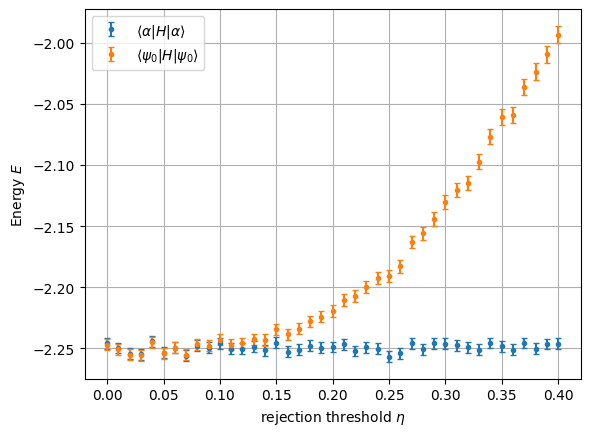
\includegraphics[width=0.73\textwidth]{img/energy.png}
		\caption{energy of actual ground state and of determined ground state for varying rejection threshold}
		\label{fig:energy}
	\end{figure}
	This is verified in Fig.~\ref{fig:energy}. The energy of the actual ground state stays constant up to statistical fluctuations. The energy of the ground states of the modified Hamiltonian increases as expected.
	
	
	\section{Dependence on the degree of the nodes}\label{sec:dependence on the degree of the nodes}
	Now, it shall be examined, whether the correctness of the detection correlates with the degree of the nodes of the graph.  To do so, many instances of the problem are generated and for each instance, the maximum, minimum and average degree over all nodes in the graph are determined. It is counted, how many detections are correct. The following diagrams are generated for a neglection threshold of 0.08.
	
	\begin{figure}[h]
		\subfloat[min. degree]{
			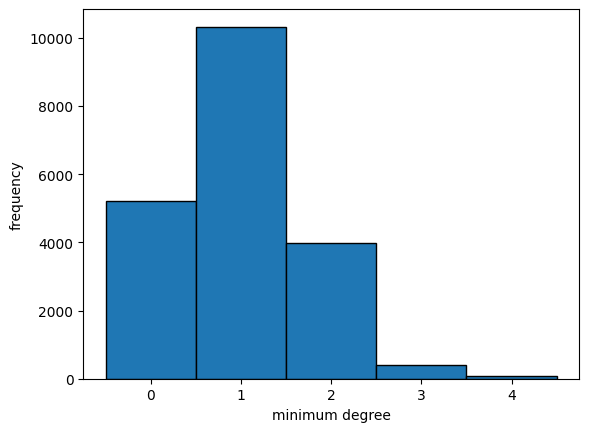
\includegraphics[width=0.33\textwidth]{img/deg_min.png}
		}
		\subfloat[avg. degree]{
			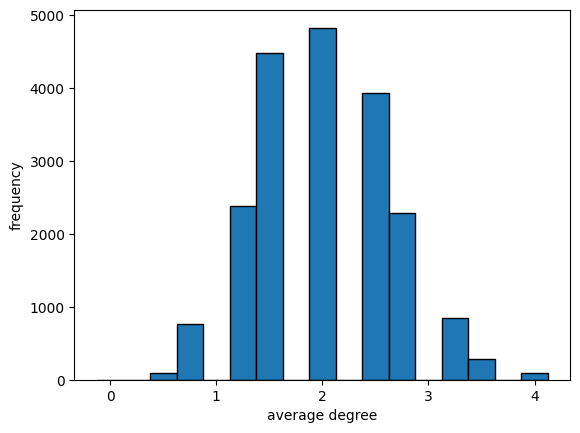
\includegraphics[width=0.33\textwidth]{img/deg_avg.png}
		}
		\subfloat[max. degree]{
			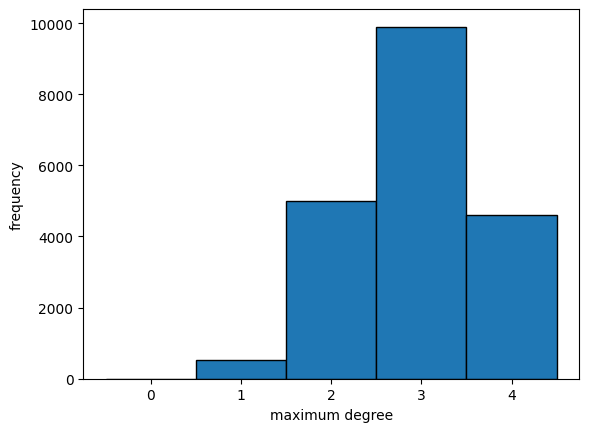
\includegraphics[width=0.33\textwidth]{img/deg_max.png}
		}
	\caption{distribution of graph counts with respect to different degrees}
	\label{fig:degrees}
	\end{figure}
	The purpose of the diagrams in Fig.~\ref{fig:degrees} is to verify how many values will be taken into consideration for each degree in order to correctly understand the following diagrams. For instance, for a {\tt neglection\_thres} of 0.08, and neglection rule 1 (threshold method), one can see that the distribution of the graph occurrences with respect to the maximum degree is approx. centered around 3, meaning that the following evaluation of correct results should yield the highest accuracy for 3 in the max. degree diagram.
	Looking at the avg. degree distribution, one notices, that there are certain average degrees which don't occur a single time. This is because they are forbidden by the topology of the graph. For instance, if $N=5$, an average degree of 1 is impossible because if there are two edges in the graph, the average degree will be $\nicefrac{4}{5}$ and if there are three edges in the graph, the avg. degree will be $\nicefrac{6}{5}$ but there will be nothing in between. 
	
	\begin{figure}[h]
		\centering
		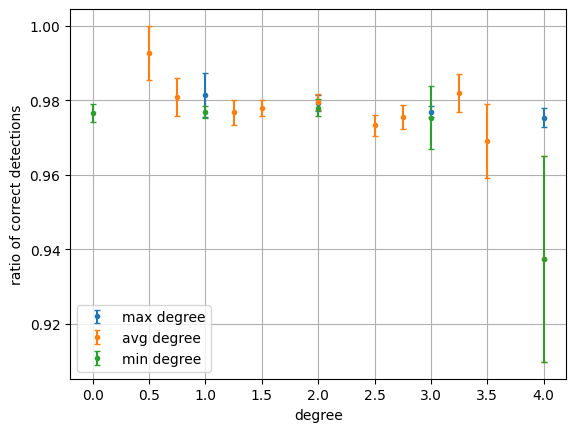
\includegraphics[width=0.75\textwidth]{img/deg_ratio.png}
		\caption{evolution of correctness ratio with respect to the degree of the nodes}
		\label{fig:correctness degree}
	\end{figure}
	The results can be seen in Fig.~\ref{fig:correctness degree}. It can be observed that the ratio of correct detections remains relatively high in the regime of over 92\,\%. For each category (min/avg/max degree) there seems to be a very slight decrease of the ratio of correct detections with increasing degree. This is counterintuitive since one would expect the correctness to increase if one allows more couplings because then there are more interactions among the qubits and the interactions in the end are what is expected to increase the correctness of the results. This effect will in the following section be observed again and an interpretation is given there. 
	
	Another observation is, that the error margins vary. For instance, considering the data points for the minimum degree, one can see that for a minimum degree of 1, the margin is the smallest while for a minimum degree of 4, the margin becomes very large. This is because of the size of the underlying data sets. As can be seen in Fig.~\ref{fig:degrees}, there are only very few generations for a minimum degree of 4 while for a minimum degree of 1, the number of generated graphs is maximal. Thus, it is evident, that the accuracy varies accordingly.   
	
	\section{Dependence on the connectedness of the graph}\label{sec:dependence on the connectedness of the graph}
	A graph is connected, if every node of the graph is connected to at least one other node of the graph. If a graph is not connected, there are at least two subgraphs of qubits not interacting with each other. One might imagine that this yields worse results than a graph describing a situation where every qubit takes part in the interaction. To test this hypothesis, many instances of problems are generated and the ground state is evaluated. For each instance it is determined, if the corresponding graph is connected or not and the evolution of the ratio of correct detections is traced. 
	
	\begin{figure}[h]
		\centering
		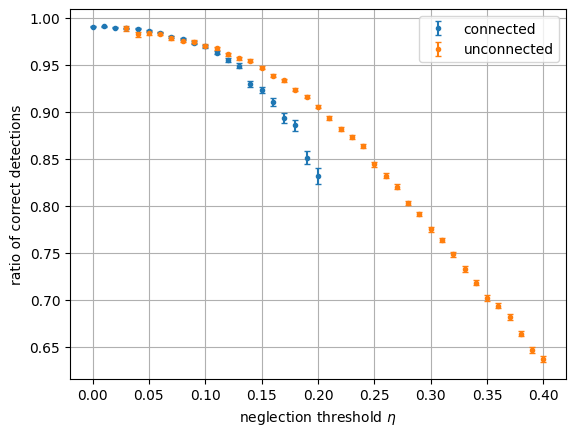
\includegraphics[width=0.75\textwidth]{img/connected_unconnected_rule_1.png}
		\caption{dependence of correct detections on the threshold for connected and unconnected graphs for the threshold method}
		\label{fig:connected unconnected rule 1}
	\end{figure}
	This ratio can be seen in Fig.~\ref{fig:connected unconnected rule 1}. As the rejection threshold increases, the ratio of correct detections drops as expected. What however is surprising, is that for larger rejection thresholds, the ratio of correct detections is dropping faster for connected graphs than for non-connected graphs. We suspect this is not because the property of having a connected graph leads to worse results but rather that the connectedness is a measure of how difficult the problem we are trying to solve really is. In other words, we achieve a lower ratio of correct solutions for connected graphs because the AUD problems that correspond to connected graphs are more difficult to solve than those corresponding to non-connected graphs. This is plausible, because a coupling is computed as $J_{ij} = -\frac{1}{2}|\vec p_i^\dagger \vec p_j|^2$. This means, if the two pilot sequences $\vec p_i$ are very similar, the corresponding coupling will be large. In a connected graph, enough couplings are at least as large as necessary not to get neglected, which only happens if the pilot sequences are similar. And if the pilot sequences are similar, it es easy to guess one bit wrong. 
	
	Further it can be observed that for $\eta>0.2$, no data points are on the curve for the connected graphs anymore. This is because for those rejection thresholds, it is very unlikely to generate a connected graph as shown in Fig.~\ref{fig:N connected rule 1}.
	
	 	
	\begin{figure}[h]
		\subfloat[number method]{
			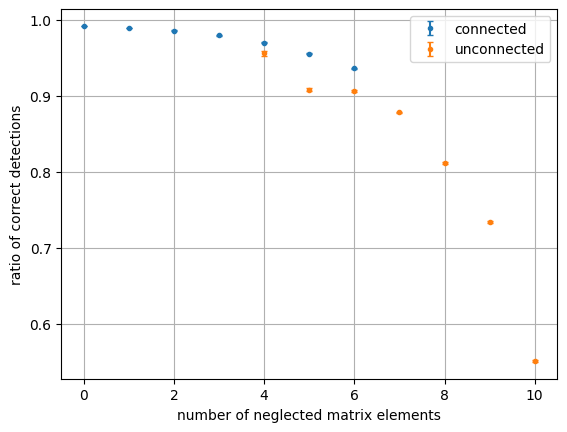
\includegraphics[width=0.49\textwidth]{img/connected_unconnected_rule_2.png}
		}
		\subfloat[max degree method]{
			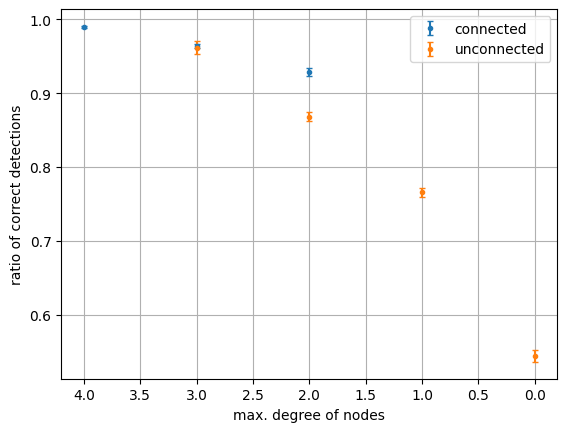
\includegraphics[width=0.49\textwidth]{img/connected_unconnected_rule_3.png}
		}
	\caption{ratio of correct detections for both other methods}
	\label{fig:connected unconnected rule 2 and 3}
	\end{figure}
For rejection rules 2 and 3, the results are shown in Fig.~\ref{fig:connected unconnected rule 2 and 3}. In contrast to the threshold method from Fig.~\ref{fig:connected unconnected rule 1}, the connected graphs seem to yield better results. To explain this observation, an examination and comparison of the coupling matrix in those cases with the coupling matrix for the first case would be necessary. 

\section{Comparison of different rejection methods}\label{sec:comparison of rejection methods}
To compare and to judge, which of the three methods is more favorable, one has to find a diagram with a common $x$-axis. This parameter is chosen to be the (average) number of neglected couplings. For the number method it is obvious how to obtain this quantity - it is simply the number of rejected matrix elements, no averaging necessary. For the threshold method, the rejection threshold is swept and for each threshold, multiple runs are conducted. The number of neglected matrix elements is tracked and after all repetitions averaged for the selected threshold. For the degree method, the maximum allowed degree is swept and the same averaging procedure is employed. 

\begin{figure}[h]
	\centering
	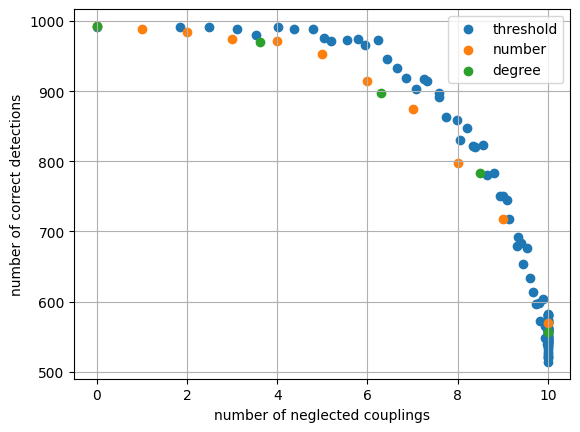
\includegraphics[width=0.75\textwidth]{img/method_comparison_correct_ratio.png}
	\caption{ratio of correct detections for three different methods of coupling rejection}
	\label{fig:method comparison correct ratio}
\end{figure}
The results are presented in Fig.~\ref{fig:method comparison correct ratio} where the number of correct detections is shown against the number of neglected couplings. It can be seen that all methods yield very similar results for 0 and 10 neglected couplings. This is to be expected, because the resulting graphs are independently of the method either the full graph or a graph, where all couplings are rejected. In between 4 and 6 neglected matrix elements, the curves of the number and the degree method seem to follow a similar course whereas the data points of the threshold method show larger values. This suggests, that for a given number of couplings that should be rejected, it is better to use the threshold method with a threshold that corresponds to this required number of matrix elements to neglect rather than to use either of the other two methods. The implications for a practical implementation however seem questionable, because a practical implementation always has to be done on an existing hardware where exactly those restrictions considered in the degree method apply. If a qubit requires more couplings than available on the quantum computer, an embedding is required where this qubit is represented using multiple qubits satisfying the stronger degree restriction which will again increase the error rate due to the increased complexity. 

\begin{figure}[h]
	\centering
	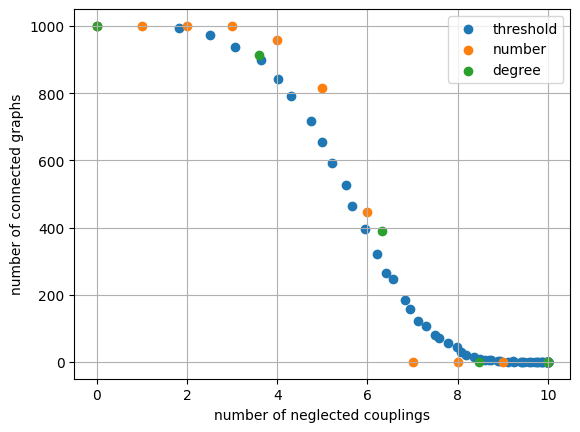
\includegraphics[width=0.75\textwidth]{img/method_comparison_connected_ratio.png}
	\caption{ratio of connected graphs for three different methods of coupling rejection}
	\label{fig:method comparison connected ratio}
\end{figure}
Furthermore, the number of connected graphs has been examined in Fig.~\ref{fig:method comparison connected ratio}. It can be seen, that in the region between 4 and 6 neglected couplings, the number method yields the highest amount of connected graphs. This however does not seem to correlate with an increased amount of correct detections and as in Sec.~\ref{sec:dependence on the connectedness of the graph} discussed, the relationship between connectedness and correct detections might be impacted by other effects, like a "preselection" of problems. Thus, it seems questionable whether the property of connectedness of a graph has any relevance at all for the AUD scenario discussed in this project. 


\section{Summary and outlook}\label{sec:summary and outlook}
In this project, three methods to reject matrix elements in the coupling matrix for the Ising model for active user detection are examined. 

The hamming distance between the determined and the actual solution of the AUD-problem is subject of Sec.~\ref{sec:hamming distance}. The progressive rejection of couplings leads to a gradual decrease in accuracy. The plateau of the ratio of correct detections coincides with the absence of couplings, the curvature seems to coincide with the number of connected graphs. In Sec.~\ref{sec:comparison with CCR} it is demonstrated, that in the case of rejection of all couplings, the result of the annealing process is equal to the result of a conventional correlation receiver for its optimal parameter choice. The modification of the coupling matrix leads to the expected increase in ground state energy as seen in Sec.~\ref{sec:energy}. Sec.~\ref{sec:dependence on the degree of the nodes} shows that there is almost no or only a very slight dependence of the ratio of correct detections on the degree of the nodes. The property of connectedness examined in Sec.~\ref{sec:dependence on the connectedness of the graph} leads to the counterintuitive finding that a connected graph seems to result in worse outcomes than a non-connected graph. This however is most likely a consequence of the fact, that connected graphs represent more difficult problems. Finally in Sec.~\ref{sec:comparison of rejection methods}, a comparison between the three methods suggests, that the threshold method yields for a given number of couplings to neglect, better results than the number- and the degree-method.
\\\\
In Ref.~\cite{PirGanGou25} we were able to show, that the application of the threshold method indeed results in a better accuracy of the experimental results in comparison to the full problem. This project suggests, that this threshold method yields better results in comparison to the number- and the degree method. In the future it would be interesting to see if this difference can be reproduced using a real quantum annealer. 
	
	
\begin{thebibliography}{9}
	\bibitem{PirGou1}R.~Piron, C.~Goursaud, ``Quantum Annealing for Active User Detection in NOMA Systems'', ACSSC 2024 - 58th Asilomar Conference on Signals, Systems, and Computers, Oct 2024, Pacific Grove
	(CA), United States. pp.1-5. 
	
	\bibitem{PirGanGou25}R.~Piron, F.~Ganzer, C.~Goursaud, ``Simplified Embedding Scheme for Quantum
	Annealing Applied to Activity Detection'', INFOCOM 2025 - International Conference on Computer Communications, London, United Kingdom.
\end{thebibliography}
	
	
\end{document}